%% -*- LaTeX -*- This is LaTeX2e code

\section{Space-Efficient Divide-and-Conquer}

In this section, we describe a simple scheme for space-efficiently
performing divide-and-conquer.  Using the standard recursive approach
requires \Wm{\log n} pointers for maintaining a recursion stack as
noted in the context of space-efficiently implementing the Quicksort
algorithm \cite{huang:one-way,wegner:generalized}. Our technique
traverses the recursion tree in the same manner without requiring the
extra pointers. In many cases, the same type of result can be obtained
using bottom-up merge, however, it is well known that bottom-up merge
has poor performance in the presence of caches.

The main idea (which is probably folklore, even though we have not
seen it in the literature) is to simulate a post-order traversal of
the recursion tree. We assume for simplicity that the data to be
processed is stored in an array \texttt{A} of size $n = 2^k$ for some
positive integer $k$. The recursion tree corresponding to a
divide-and-conquer scheme is a perfectly balanced binary tree, in
which each node at depth $0 \leq i < k$ corresponds to a subarray of
the form \texttt{A}$[j \cdot 2^{k-i} \ldots (j + 1) \cdot 2^{k-i} -
1]$ for some integer $0 \leq j \leq i$.\footnote{If the problem size
  is not an exact power of two, we imagine the recursion tree to be
  embedded into a perfectly balanced tree and stop traversing the tree
  prematurely.}

Our scheme is presented in Algorithm~\ref{alg:traversal}. We maintain
two indices $b$ and $e$ that indicate the subarray \texttt{A}$[b
\ldots e-1]$ currently processed. We will use the binary
representation of the index $e$ to implicitly store the current status
of the post-order traversal, i.e., the node of the simulated recursion
tree currently visited.

\begin{algorithm}
  \caption{Stackless simulation of post-order traversal.}
  \label{alg:traversal}
  \begin{algorithmic}[1]
    \STATE Let $b=0$ and $e=1$.
    \WHILE{$b\neq 0$ or $e\leq n$}
    \STATE \{Process all items in $\texttt{a}[b\ldots e-1]$.\}
    \STATE Let $i$ be the index of the least significant bit of $e$
    (note that the lowest index is $0$).
    \FOR{$c:=1$ to $i$}
    \STATE Set $b := e-2^c$.
    \STATE Merge the two subarrays in $\texttt{a}[b\ldots e-1]$
    \ENDFOR 
    \STATE Let $e := e + 1$.
    \ENDWHILE
  \end{algorithmic}
\end{algorithm}

Determining the value of $i$ (Step 3) can be done in \Oh{1} amortized
time without extra space using a straightforward implementation of a
binary counter.

The above algorithm basically traverses the ``recursion tree'' left to
right. When processing a leaf $v$, the algorithm backtracks in
geomtrically increasing steps merging all subtrees already traversed
completely. This merging is done by traversing a leaf-to-root path
starting from $v$ but stopping as soon as the path goes up to the
right (Figure~\ref{fig:tree_spaceefficient}). The correctness of the
algorithm follows from the next lemma:\ournote{JV: Do we need a
  proof?}

\begin{lemma}
  If the leaves of a complete binary tree are labeled from left to
  right (starting with $1$ for the leftmost leaf), the height of the
  largest subtree containing the leaf $e>1$ as its rightmost leaf is
  equal to the index $i$ of the least significant bit of the number
  $e$.
\end{lemma}

\begin{figure}
  \centerline{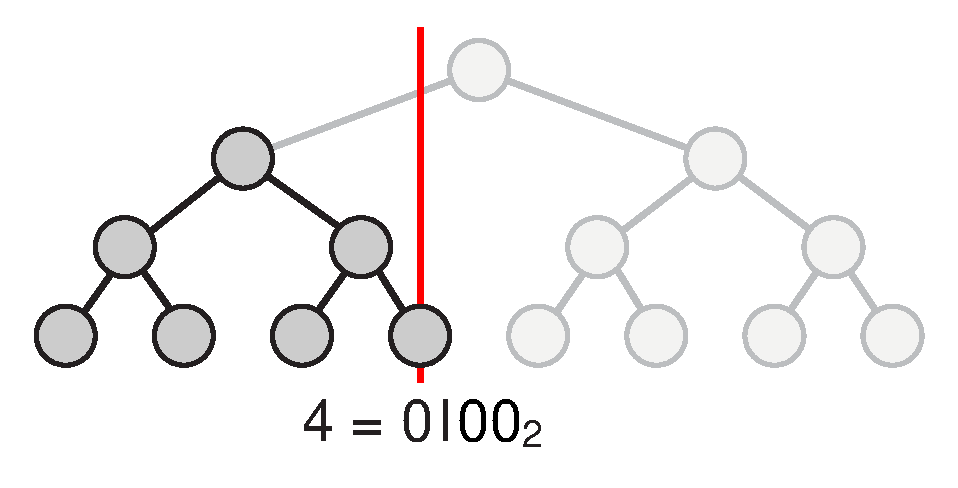
\includegraphics[height=3.5cm]{tree_spaceefficient}}
  \caption{Merging subtrees while traversing left-to-right.}
  \label{fig:tree_spaceefficient}
\end{figure}

%%% Local Variables:
%%% mode: latex
%%% TeX-master: "paper"
%%% End:
